\documentclass[a4]{article}
\pagestyle{myheadings}

%%%%%%%%%%%%%%%%%%%
% Packages/Macros %
%%%%%%%%%%%%%%%%%%%
\usepackage{mathrsfs}



\usepackage{fancyhdr}
\pagestyle{fancy}
\lhead{}
\chead{}
\rhead{}
\lfoot{}
\cfoot{} 
\rfoot{\normalsize\thepage}
\renewcommand{\headrulewidth}{0pt}
\renewcommand{\footrulewidth}{0pt}
\newcommand{\RomanNumeralCaps}[1]
    {\MakeUppercase{\romannumeral #1}}

\usepackage{amssymb,latexsym}  % Standard packages
\usepackage[utf8]{inputenc}
\usepackage[russian]{babel}
\usepackage{MnSymbol}
\usepackage{mathrsfs}
\usepackage{amsmath,amsthm}
\usepackage{indentfirst}
\usepackage{graphicx}%,vmargin}
\usepackage{graphicx}
\graphicspath{{pictures/}} 
\usepackage{verbatim}
\usepackage{color}
\usepackage[nottoc,numbib]{tocbibind}
\usepackage{float}

\usepackage{listings}
\definecolor{codegreen}{rgb}{0,0.6,0}
\definecolor{codegray}{rgb}{0.5,0.5,0.5}
\definecolor{codepurple}{rgb}{0.58,0,0.82}
\definecolor{backcolour}{rgb}{0.95,0.95,0.92}
 
\lstdefinestyle{mystyle}{
    backgroundcolor=\color{backcolour},   
    commentstyle=\color{codegreen},
    keywordstyle=\color{magenta},
    numberstyle=\tiny\color{codegray},
    stringstyle=\color{codepurple},
    basicstyle=\footnotesize,
    breakatwhitespace=false,         
    breaklines=true,                 
    captionpos=b,                    
    keepspaces=true,                 
    numbers=left,                    
    numbersep=5pt,                  
    showspaces=false,                
    showstringspaces=false,
    showtabs=false,                  
    tabsize=2
}
 
\lstset{style=mystyle}

\usepackage{url}
\urldef\myurl\url{foo%.com}





\DeclareGraphicsExtensions{.pdf,.png,.jpg}% -- настройка картинок

\usepackage{epigraph} %%% to make inspirational quotes.
\usepackage[all]{xy} %for XyPic'a
\usepackage{color} 
\usepackage{amscd} %для коммутативных диграмм
%\usepackage[colorlinks,urlcolor=red]{hyperref}

%\renewcommand{\baselinestretch}{1.5}
%\sloppy
%\usepackage{listings}
%\lstset{numbers=left}
%\setmarginsrb{2cm}{1.5cm}{1cm}{1.5cm}{0pt}{0mm}{0pt}{13mm}


\newtheorem{Lemma}{Лемма}[section]
\newtheorem{Proposition}{Предложение}[section]
\newtheorem{Theorem}{Теорема}[section]
\newtheorem{Corollary}{Следствие}[section]
\newtheorem{Remark}{Замечание}[section]
\newtheorem{Definition}{Определение}[section]
\newtheorem{Designations}{Обозначение}[section]




%%%%%%%%%%%%%%%%%%%%%%% 
%Подготовка оглавления% 
%%%%%%%%%%%%%%%%%%%%%%% 
\usepackage[titles]{tocloft}
\renewcommand{\cftdotsep}{2} %частота точек
\renewcommand\cftsecleader{\cftdotfill{\cftdotsep}}
\renewcommand{\cfttoctitlefont}{\hspace{0.38\textwidth} \LARGE\bfseries} 
\renewcommand{\cftsecaftersnum}{.}
\renewcommand{\cftsubsecaftersnum}{.}
\renewcommand{\cftbeforetoctitleskip}{-1em} 
\renewcommand{\cftaftertoctitle}{\mbox{}\hfill \\ \mbox{}\hfill{\footnotesize Стр.}\vspace{-0.5em}} 
%\renewcommand{\cftchapfont}{\normalsize\bfseries \MakeUppercase{\chaptername} } 
%\renewcommand{\cftsecfont}{\hspace{1pt}} 
\renewcommand{\cftsubsecfont}{\hspace{1pt}} 
%\renewcommand{\cftbeforechapskip}{1em} 
\renewcommand{\cftparskip}{3mm} %определяет величину отступа в оглавлении
\setcounter{tocdepth}{5} 
\renewcommand{\listoffigures}{\begingroup %добавляем номер в список иллюстраций
\tocsection
\tocfile{\listfigurename}{lof}
\endgroup}
\renewcommand{\listoftables}{\begingroup %добавляем номер в список иллюстраций
\tocsection
\tocfile{\listtablename}{lot}
\endgroup}


   
   
%\renewcommand{\thelikesection}{(\roman{likesection})}
%%%%%%%%%%%
% Margins %
%%%%%%%%%%%
\addtolength{\textwidth}{0.7in}
\textheight=630pt
\addtolength{\evensidemargin}{-0.4in}
\addtolength{\oddsidemargin}{-0.4in}
\addtolength{\topmargin}{-0.4in}

%%%%%%%%%%%%%%%%%%%%%%%%%%%%%%%%%%%
%%%%%%Переопределение chapter%%%%%% 
%%%%%%%%%%%%%%%%%%%%%%%%%%%%%%%%%%%
\newcommand{\empline}{\mbox{}\newline} 
\newcommand{\likechapterheading}[1]{ 
\begin{center} 
\textbf{\MakeUppercase{#1}} 
\end{center} 
\empline} 

%%%%%%%Запиливание переопределённого chapter в оглавление%%%%%% 
\makeatletter 
\renewcommand{\@dotsep}{2} 
\newcommand{\l@likechapter}[2]{{\bfseries\@dottedtocline{0}{0pt}{0pt}{#1}{#2}}} 
\makeatother 
\newcommand{\likechapter}[1]{ 
\likechapterheading{#1} 
\addcontentsline{toc}{likechapter}{\MakeUppercase{#1}}} 




\usepackage{xcolor}
\usepackage{hyperref}
\definecolor{linkcolor}{HTML}{000000} % цвет ссылок
\definecolor{urlcolor}{HTML}{AA1622} % цвет гиперссылок
 
\hypersetup{pdfstartview=FitH,  linkcolor=linkcolor,urlcolor=urlcolor, colorlinks=true}

%%%%%%%%%%%%
% Document %
%%%%%%%%%%%%

%%%%%%%%%%%%%%%%%%%%%%%%%%%%%
%%%%%%главы -- section*%%%%%%
%%%%section -- subsection%%%%
%subsection -- subsubsection%
%%%%%%%%%%%%%%%%%%%%%%%%%%%%%
\def \newstr {\medskip \par \noindent} 



\begin{document}
\def\contentsname{\LARGE{Содержание}}
\thispagestyle{empty}
\begin{center} 
\vspace{2cm} 
{\Large \sc Санкт-Петербургский Политехнический}\\
\vspace{2mm}
{\Large \sc Университет} им. {\Large\sc Петра Великого}\\
\vspace{1cm}
{\large \sc Институт прикладной математики и механики\\ 
\vspace{0.5mm}
\textsc{}}\\ 
\vspace{0.5mm}
{\large\sc Кафедра прикладной математики}\\
\vspace{15mm}
%\rule[0.5ex]{\linewidth}{2pt}\vspace*{-\baselineskip}\vspace*{3.2pt} 
%\rule[0.5ex]{\linewidth}{1pt}\\[\baselineskip] 
{\huge \sc Лабораторная работа №$5$\\
\vspace{4mm}
Эмиссионная томография плазмы.\\
\vspace{4mm}
Решение ИСЛАУ
\vspace{6mm}
 }
\vspace*{2mm}
%\rule[0.7ex]{\linewidth}{1pt}\vspace*{-\baselineskip}\vspace{3.2pt} 
%\rule[0.5ex]{\linewidth}{2pt}\\ 
\vspace{1cm}

{\sc $4$ курс$,$ группа $3630102/60201$}

\vspace{2cm} 
Студент \hfill Д. А. Плаксин\\
\vspace{1cm}
Преподаватель \hfill Баженов А. Н.\\
\vspace{20mm} 

\end{center} 
%\author{Я}
\begin{center}
\vfill {\large\textsc{Санкт-Петербург}}\\ 
2019 г.
\end{center}

%%%%%%%%%%%%%%%%%%%%%%%%%%%%%%%%%%%%%%%%%%%%%%%%%%%%%%%%%%%%%%%%%%%%%%%%%%%%%%%%%%%%%%%%%%%%%%
%\ \\[4cm]

%\rm
%%%%%%%%%%%%%%%%%%%%%%%%%%%%%%%%%%%%%%%%%%%%%%%%%%%%%%%%%%%%%%%%%%%%%%%%%%%%%%%%%%%%%%%%%%%%%%
\newpage
\pagestyle{plain}

%\begin{center}
%\begin{abstract} 

%\end{abstract}

%\end{center}
\newpage
\tableofcontents{}
\newpage
\listoffigures{}
\newpage

\section{Постановка задачи}
Считать данные правой части – значения детектора

Решить полученную в лабораторной $№4$ СЛАУ различными способами:

\begin{enumerate}
    \item $x=(A^tA)^{-1}A^tb$
    \item используя функцию $tolsolvty$ \hfill\cite{tolsolvty}
\end{enumerate}


\section{Теория}
Для построение ИСЛАУ представим правую часть уравнения $Ax=b$ как интервал $Ax = [ \underline b, \overline b]$

Рассматриваются показатели детектора во временные интервалы с "текущий" $ \minus K$ до "текущий" + К

$\underline b\;\--$ минимум $b$ в некотором окне радуиса $K$

$\overline b\;\--$ максимум $b$ в некотором окне радиуса $K$

Матрицу $A$ оставляем исходной

Функция $tolsolvty$ возвращает:
\begin{itemize}
    \item $tolmax\;\--$ значение максимума распознающего функционала
    \item $argmax\;\--$ доставляющий его вектор значений аргумента, который лежит в допусковом множестве решений при $tolmax\geq 0,$ (остальные возвращаемые значения нас сейчас не интересуют)
\end{itemize}

Если $tolmax<0,$ то допусковое множество решений интервальной линейной системы пусто.

Тогда ослабим условия. Для этого расширим интервал $[\underline b,\overline b]$ так, чтобы допусковое решение было не пусто.

$$\underline b =\underline b -\Delta b$$
$$\overline b = \overline b + \Delta b$$

Для получения решения достаточно взять $\Delta b = \vert tolmax\vert$





\section{Реализация}
Все задания были выполнены на языке программирования $Matlab$ в среде разработки $MATLAB R2014b$ \hfill \cite{1}

Данные о расположении и параметрах детектора взяты пособия к лабораторной работе \hfill\cite{source2}

Значения детектора записаны в файле, полученном от преподавателя

Функция tolsolvty \hfill \cite{tolsolvty}

Для вычисления числа обусловленности интервальной матрицы используется функция $HeurMinCond,$ полученная от преподавателя

\section{Результаты}

Рассматривается набор данных $37000,$ временной интервал $000162,$ матрица $A$ размерности $256\times 174$

Число обусловленности матрицы $A:\;cond(A)=8.2719\cdot 10^{31}$

Число обусловленности матрицы $A^tA:\;cond(A^tA)=5.2939\cdot 10^{35}$


\subsection{Решение МНК}
Первый способ решения:
$$x=(A^tA)^{-1}A^tb$$

Так как матрица $A$ сильно разрежена, собственные числа квадратной матрицы $A^tA$ сконцентрированы около нуля.
\begin{figure}[H]
\begin{center}
\caption{Гистограмма собственных чисел матрицы $A^tA$}
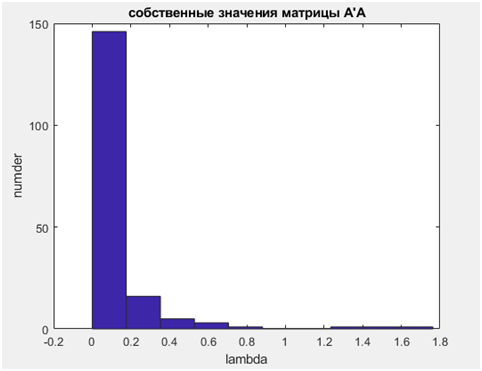
\includegraphics{pic1.png} 
\end{center}
\end{figure}

Всего $23$ собственных числа больше $0.2$
В качестве решения Matlab`ом получен вектор, состоящий из NaN (т.к. число обусловленности столь большое надежда на нахождение обратной матрицы почти отсутствует)

\subsection{Функция $tolsolvty$}
Для нахождения интервала $b$ выбрано "окно" с радиусом $K=1.$

При первой попытке нахождения решения было получено значение $tolmax = -16.0667.$

Так как $tolmax < 0,$ то допусковое множество решений интервальной системы пусто.

\begin{figure}[H]
\begin{center}
\caption{График первой попытки решения}
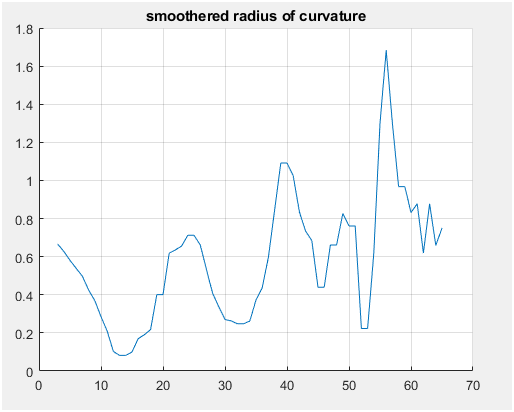
\includegraphics{pic2.png} 
\end{center}
\end{figure}


Теперь выберем $\Delta b = 16.0667,$ тем самым расширив границы $b.$

Для второй попытки нахождения решения получаем, что $tolmax=0,$ следовательно допусковое множество решений интервальной линейной системы непусто.

\begin{figure}[H]
\begin{center}
\caption{График решения с расширенным интервалом}
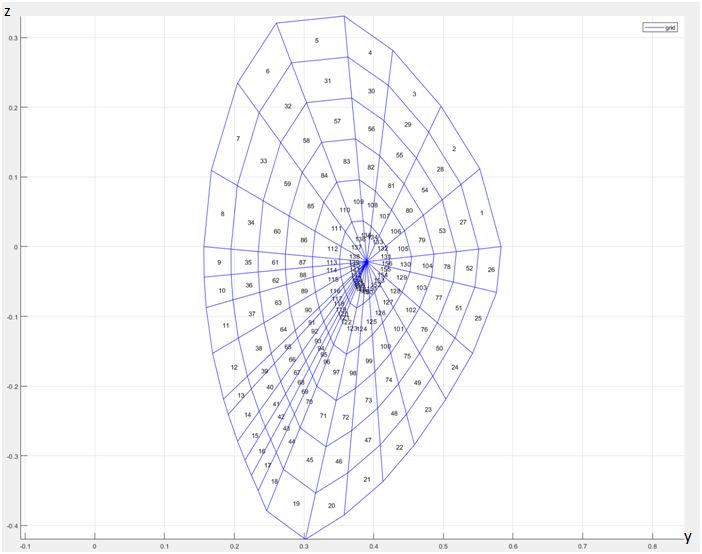
\includegraphics{pic3.png} 
\end{center}
\end{figure}

Полученное решение:

\begin{figure}[H]
\begin{center}
\caption{График полученного решения от $i$}
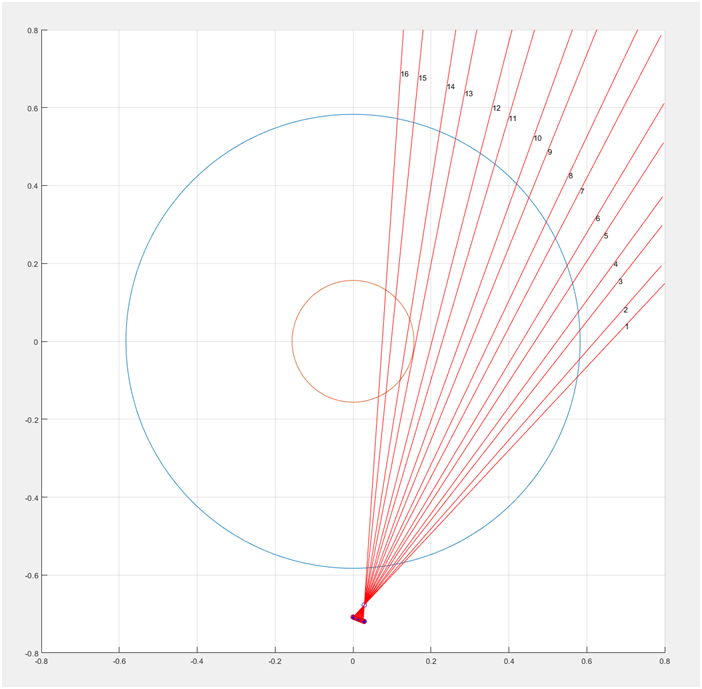
\includegraphics{pic4.png} 

\caption{Гистограмма решения, полученного с помощь $tolsolvty$}
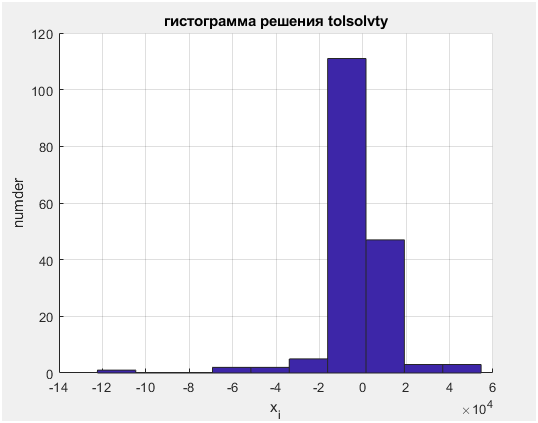
\includegraphics{pic5.png} 
\end{center}
\end{figure}

\subsection{Оценка числа обусловленности интервальной матрицы $A$}

В качестве оценки радиуса элементов матрицы $А$ возьмём $10\%$ от их величины.

Выбор именно $10\%$ обусловлен тем, что точность знания сепаратрисы, по которой построена матрицы $А$ около $10\%.$

Тогда оценка числа обусловленности интервальной матрицы $A$ равна $6.2114e+31$

Рассмотрим значения оценки числа обусловленности для разного количества повторений про постоянном радиусе элементов $10\%$

\begin{figure}[H]
\begin{center}
\caption{Значение числа обусловленности при изменении числа итераций}
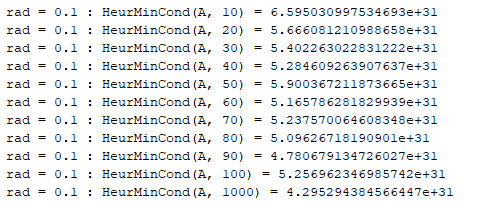
\includegraphics{pic6.png} 
\end{center}
\end{figure}

Рассмотрим значения оценки числа обусловленности для разных радиусов элементов А при постоянном числе итераций равным $100.$

\begin{figure}[H]
\begin{center}
\caption{Значение числа обусловленности при изменении радиуса элементов}
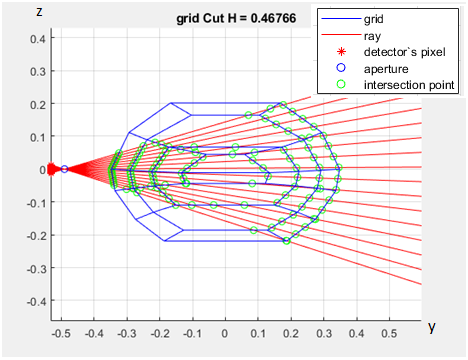
\includegraphics{pic7.png} 
\end{center}
\end{figure}

\subsection{Оценка вариабельности $IVE$}
$$IVE(A,b)=\sqrt{n} \max\limits_{\mathbb{R}^n} Tol\cdot\left(\min\limits_{A\in\mathbf{A}}cond_2A\right)\cdot\frac{\|arg\max\limits_{\mathbb{R}^n}Tol\|_2}{\|\hat{\mathbf{b}}\|_2}$$

Так как для полученного решения $maxtol=0,$ то и $IVE(A,b)=0$ \hfill\cite{source4}


\section{Обсуждение}
СЛАУ представляет собой матрицу $256\times N,$ где $N$ – это количество элементов разбиения.
Матрица $А$ имеет огромное число обусловленности $cond(A)= 8.2719\cdot 10^{31}.$ Это означает, что матрица крайне плохо обусловлена. 
Матрица $A$ – плохо обусловлена. От того матрица $A^t A$ становится уже настолько плохо обусловлена $cond(A^t A)= 5.2939\cdot 10^{35},$ что невозможно получить решение в виде: $x=(A^t A)^{-1} A^t b$
Вторым методом ИСЛАУ решение получено, но при этом сильно ослаблены условия на b (раздвинуты границы интервала). И не гарантируется, что x≥0. А изначальная постановка задачи требует, чтобы излучение было неотрицательным.



\begin{thebibliography}{}
    \bibitem{1}  Документация по Матлаб: https://www.mathworks.com/help/

    \bibitem{2} Код функции g\_file\_extractor\_1t: https://cloud.mail.ru/public/5o3T/4G4dD71hL
    
    \bibitem{source}
    Пособие к Лабораторным работам https://cloud.mail.ru/public/4ra6/5wwqBzMBC/LabPractics.pdf
    
    \bibitem{tolsolvty}
    Код функции tolsolvty http://www.nsc.ru/interval/Programing/MCodes/
    
    \bibitem{source1}
    Пособие к Лабораторным работам «Построение матриц СЛАУ» https://vk.com/doc38035266\_528474113?hash=8c9ddc720dfadef7b6\&dl=48b180ef19a7dc0f33
    
    \bibitem{source2}
    Выпуская квалификационная работа бакалавра «Исследование разрешимости обратных задач с помощью распознающего функционала» https://cloud.mail.ru/public/4ra6/5wwqBzMBC/2019\%20\%D0\%97\%D0\%B0\%D1\%82\%D1\%8B\%D0\%BB\%D0\%BA\%D0\%B8\%D0\%BD\%20\%D0\%B1\%D0\%B0\%D0\%BA\%D0\%B0\%D0\%BB\%D0\%B0\%D0\%B2\%D1\%80.pdf
    
    \bibitem{source4}
    О мере вариабельности оценки параметров в статистике интервальных данных» http://www-sbras.nsc.ru/interval/shary/Papers/SShary-VariabMeasure-JCT.pdf
    
\end{thebibliography}

\section{Приложения}

Код отчёта:\; \url{https://github.com/MisterProper9000/computing-complex/blob/Lab-5(interval-linear-system)/Lab_5(interval_linear_system)/texReport/lab4.tex}

Код лаборатрной:\; \url{https://github.com/MisterProper9000/computing-complex/blob/Lab-5(interval-linear-system)/Lab_5(interval_linear_system)}



\end{document}